\section{System Architecture and Execution Details}
\label{sec:system}
AgentGS implements the method through an interactive frontend, an orchestration service, registered knowledge resources, and a tool execution service (Figure~\ref{fig:architecture}). This appendix describes how the plan in \papersection{sec:method}{3} becomes an inspectable sequence of calls.
\begin{figure*}[t]
  \centering
  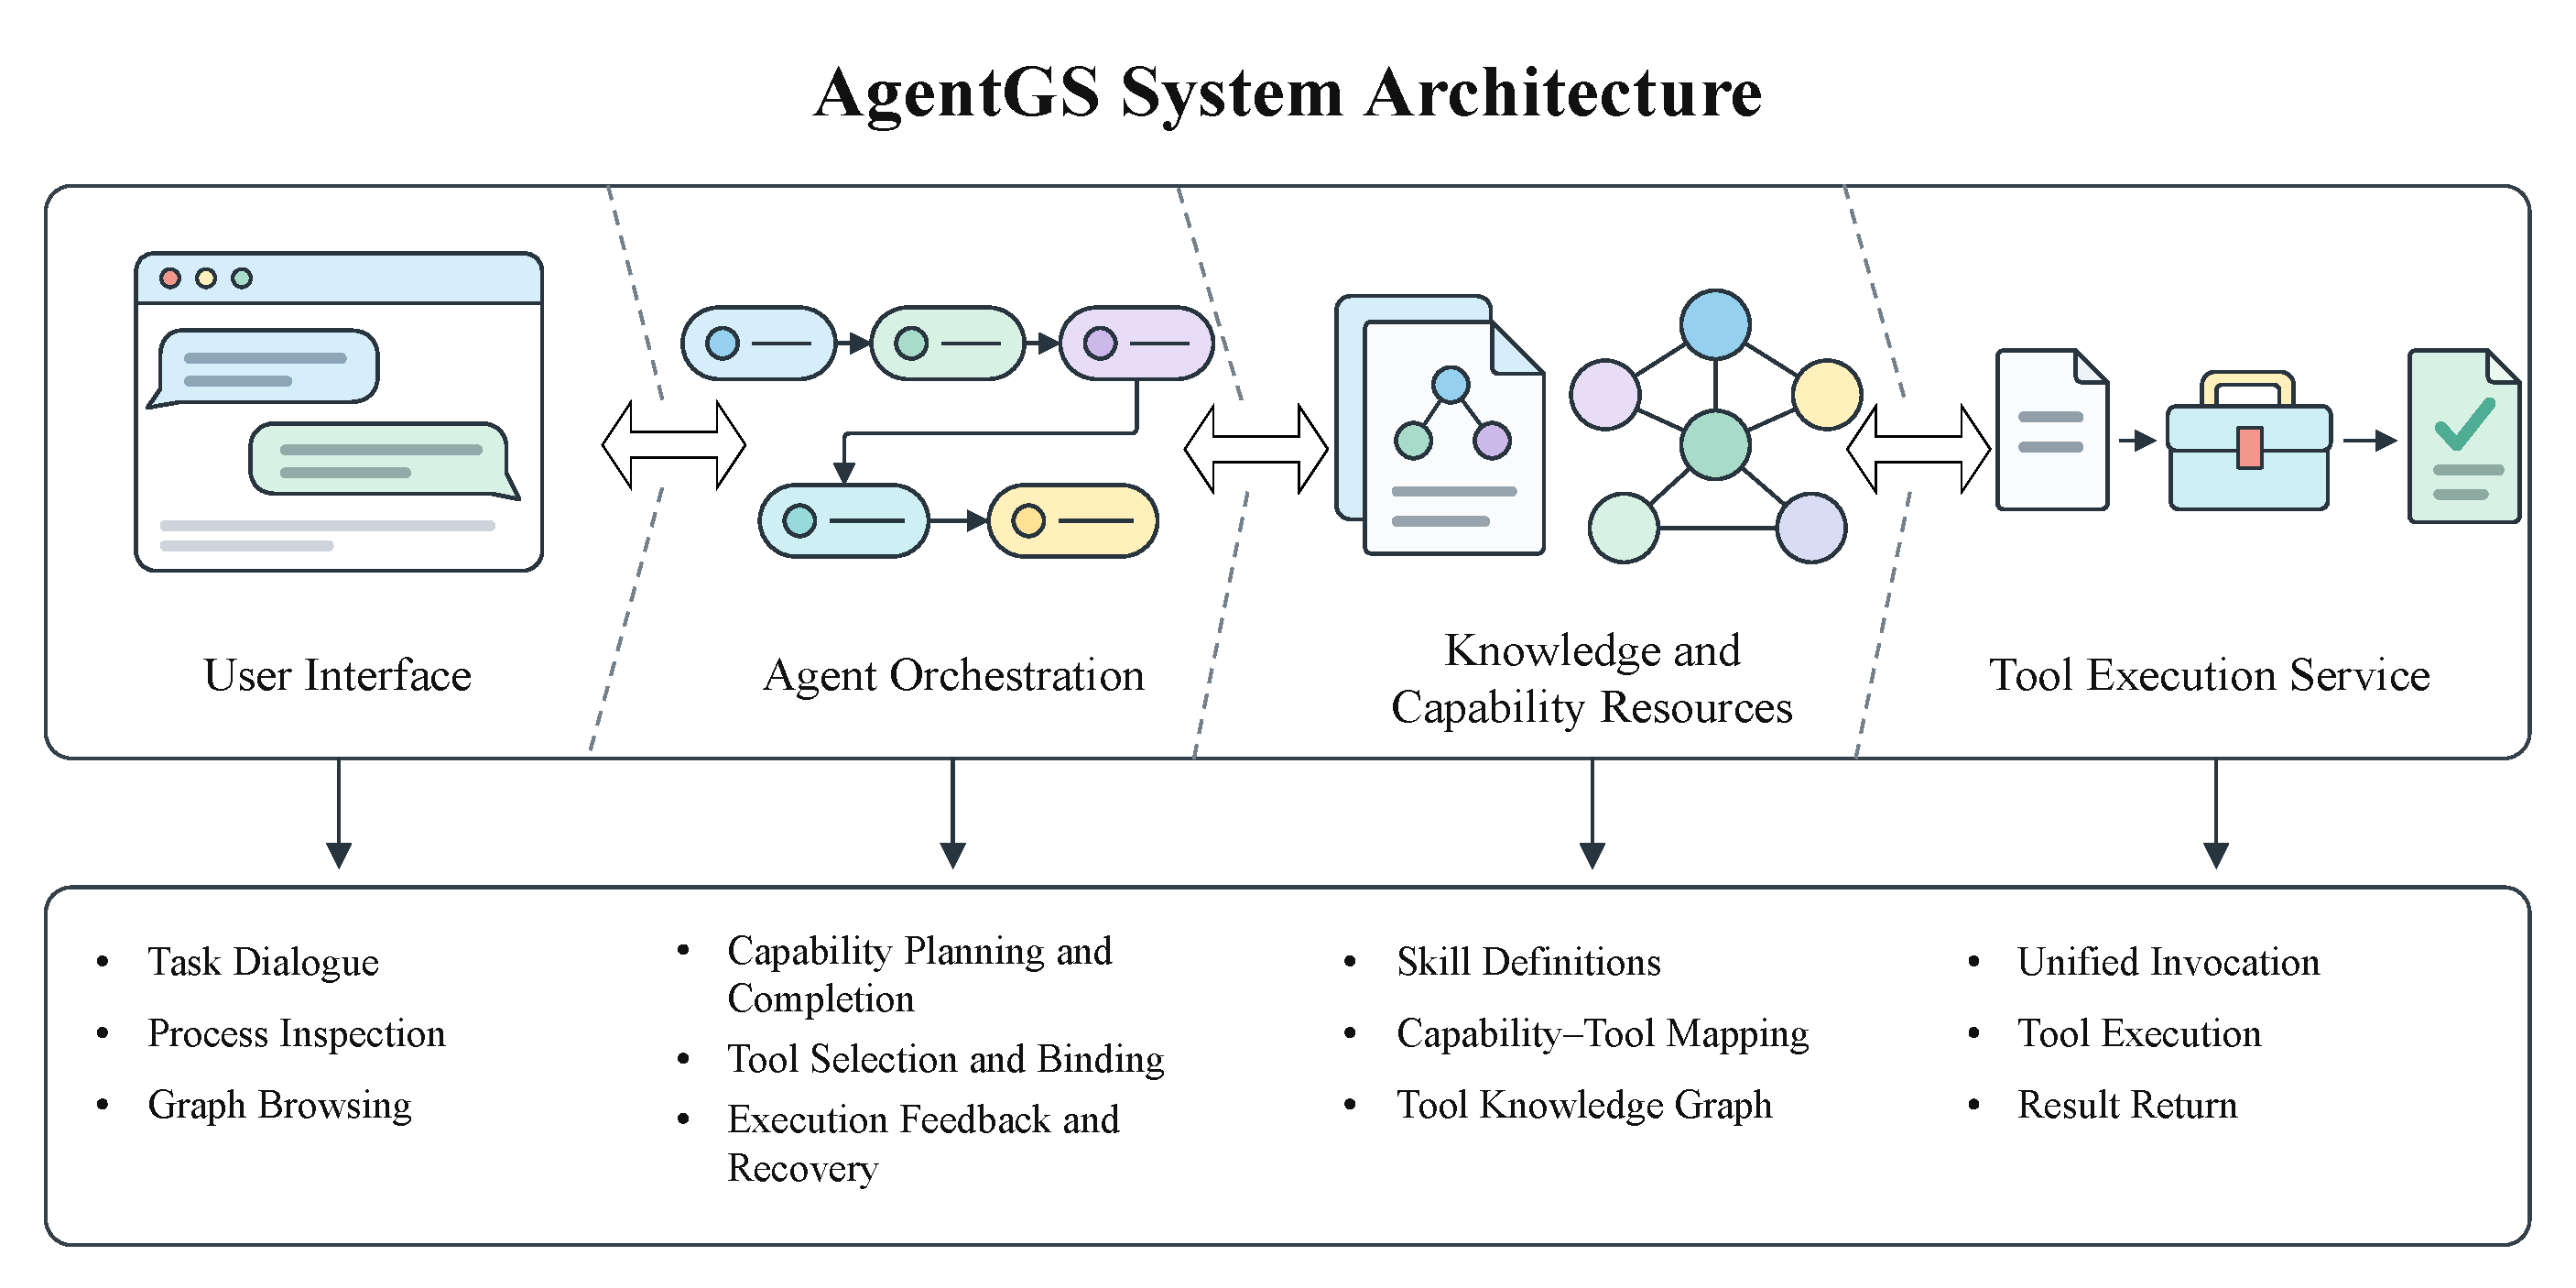
\includegraphics[width=\textwidth]{fig_architecture.pdf}
  \caption{AgentGS architecture and main functions. The system comprises an interactive frontend, an agent orchestration service, knowledge and capability resources, and a tool execution service.}
  \label{fig:architecture}
  \Description{The user interface exchanges tasks and results with orchestration. Orchestration accesses Skill definitions, capability-to-tool mappings, and tool knowledge graphs, and delegates concrete invocations to the tool execution service.}
\end{figure*}


\subsection{Separation of Planning and Execution}
The frontend accepts questions and resources and displays the returned answer and execution records. Orchestration retrieves strategies and tools, prepares capability requirements, invokes model planning, and validates the resulting instances. Knowledge resources provide Skill declarations, capability mappings, and tool descriptions. The execution service invokes a registered interface and returns its observed output or failure.

This separation allows planning to reason over declared operations while execution operates on concrete argument objects. Descriptive similarity between two tools does not by itself authorize substitution: the capability occurrence's scope and the selected interface schema still apply.

\subsection{Execution Instances and Input Bindings}
An execution step records its identity, tool, purpose, predecessor identities, literal arguments, and upstream input bindings. Optional Skill and Capability identifiers establish its declared scope. Unknown or forward dependencies and duplicate instance identities are rejected before execution.

A binding names a producing instance and a path into its observed structured output. The consumer receives the resolved value rather than an unverified description of what the producer was expected to return. Explicit references remain authoritative when arguments are repaired. This prevents a failed or inappropriate argument from being silently replaced with a convenient unrelated value.

Artifacts additionally retain provenance such as the producing step and tool. File and scalar bindings are validated according to their expected inputs. An operation on the wrong artifact may still execute successfully, which is why invocation success and reference-answer correctness are tracked separately.

\subsection{Recovery and Reuse Boundaries}
When execution recovery is enabled, the runtime can use failure feedback for argument correction and another plan attempt under configured limits. Initial model-plan repair, protocol repair, transport retries, and scientific tool retries have separate counters and scopes. Exhausting a communication budget does not establish that a scientific computation has been safely replayed.

A result can be reused across plan attempts only when the instance has unchanged semantics, fully specified inputs, and verified upstream reuse identities. The current runtime permits this for an explicit set of pure scalar computations. File-backed, implicit-input, and external-data operations are rerun rather than assumed unchanged. Matching tool names or retaining the same position in a chain is insufficient to establish reuse.

With execution recovery disabled, the first failed scientific execution ends that chain and answer generation reports incomplete work. Initial argument construction and validation remain available, so the intervention targets reaction to observed failure rather than removal of ordinary execution checks.

\subsection{Knowledge Integration and Process Inspection}
Integrating a tool registers its identifier, parameter schema, and input/output information, then associates it with relevant capabilities. A Skill supplies the strategy-specific dependency and implementation constraints. Runtime selection checks those declarations together with tool availability and the task's concrete inputs.

The interface exposes plans, invocation inputs and outputs, execution states, and failure feedback. Tool-graph browsing presents registered tools and associations as retrieval and inspection aids. These associations do not supersede capability dependencies or establish valid argument flow. Retained histories make it possible to inspect whether the intended file was read, whether the correct upstream value was consumed, and which attempts contributed to the final answer.
